
\documentclass[11pt]{article}

\usepackage{amsmath,amssymb,amsthm,physics}
\usepackage{geometry}
\usepackage{hyperref}
\usepackage{bm}
\usepackage{tensor}
\usepackage{graphicx}
\usepackage{tikz}
\usepackage{tikz-3dplot}
\usepackage{cite}
\usepackage{enumitem}

\geometry{margin=1in}

\title{\textbf{Anapoles, Gauge Constraints, and the Hidden Structure of Electrodynamics}}
\author{}
\date{}

\begin{document}

\maketitle

\begin{abstract}
We present a comprehensive treatment of anapole moments as fundamental, non-radiative degrees of freedom in classical and quantum electrodynamics. Using vector spherical harmonics, constraint analysis, and gauge theory, we show that anapoles arise naturally from the longitudinal sector of Maxwell theory and survive gauge reduction. Their relation to BRST cohomology, gravitational analogues, and the no-interaction theorem is developed. Several geometric figures illustrate the physical content.
\end{abstract}

\tableofcontents
\newpage

%========================================================
\section{Introduction}

Electromagnetic theory is usually interpreted in terms of radiation and particle interactions. 
However, Maxwell theory possesses physical field configurations that neither radiate nor reduce to gauge artifacts.
These configurations — known as \emph{anapoles} — represent genuine physical structure encoded in the constraint sector of gauge theory.

This work provides a unified treatment of these degrees of freedom using modern geometric and field-theoretic methods.

%========================================================
\section{Maxwell Theory as a Constrained System}

The action is
\begin{equation}
S = -\frac14 \int F_{\mu\nu}F^{\mu\nu}\, d^4x + \int J^\mu A_\mu\, d^4x,
\end{equation}
with
\begin{equation}
F_{\mu\nu} = \partial_\mu A_\nu - \partial_\nu A_\mu.
\end{equation}

Gauge invariance:
\begin{equation}
A_\mu \rightarrow A_\mu + \partial_\mu \chi.
\end{equation}

Gauss law:
\begin{equation}
\nabla \cdot \mathbf{E} = \rho.
\end{equation}

This is a constraint, not a dynamical equation.

%========================================================
\section{Vector Spherical Harmonics}

Define scalar harmonics \(Y_{lm}\). Then:

\begin{align}
\mathbf{Y}_{lm} &= Y_{lm}\hat{r}, \\
\mathbf{\Psi}_{lm} &= r\nabla Y_{lm}, \\
\mathbf{\Phi}_{lm} &= \hat{r} \times \nabla Y_{lm}.
\end{align}

\begin{center}
\begin{tabular}{c|c|c|c}
Mode & Divergence & Curl & Parity \\ \hline
$\mathbf{Y}_{lm}$ & $\neq 0$ & $0$ & $(-1)^l$ \\
$\mathbf{\Psi}_{lm}$ & $\neq 0$ & $\neq 0$ & $(-1)^l$ \\
$\mathbf{\Phi}_{lm}$ & $0$ & $\neq 0$ & $(-1)^{l+1}$
\end{tabular}
\end{center}

Any vector field decomposes as:
\[
\mathbf{A} = \sum_{lm}
\left(
a_{lm}\mathbf{Y}_{lm}
+ b_{lm}\mathbf{\Psi}_{lm}
+ c_{lm}\mathbf{\Phi}_{lm}
\right).
\]

%========================================================
\section{Toroidal (Anapole) Modes}

Anapole configurations correspond to:
\[
\mathbf{A}_{\text{ana}} = \nabla \left( g_l(r) Y_{lm} \right).
\]

They are pure gauge outside sources but physical within them.

\subsection*{Anapole Moment}

\begin{equation}
\boxed{
\mathbf{a} = \frac{1}{10}
\int d^3r
\left[
r^2 \mathbf{J}
- 3\mathbf{r}(\mathbf{r}\cdot\mathbf{J})
\right]
}
\end{equation}

Equivalent form:
\[
\mathbf{a} = \frac12 \int \mathbf{r} \times (\mathbf{r} \times \mathbf{J})\, d^3r.
\]

---

%========================================================
\section{Why Anapoles Do Not Radiate}

Radiation depends on:
\[
\int \mathbf{J}, \quad \int \mathbf{r}\times\mathbf{J}.
\]

Anapoles satisfy:
\[
\int \mathbf{J} = 0, \qquad \int \mathbf{r}\times\mathbf{J} = 0.
\]

Hence no far-field radiation exists.

---

%========================================================
\section{Geometric Interpretation (Figure)}

\begin{figure}[h!]
\centering
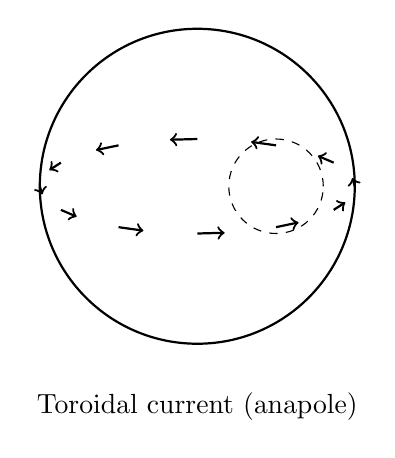
\begin{tikzpicture}[scale=2]

% torus
\draw[thick] (0,0) circle (1);
\draw[dashed] (0.5,0) circle (0.3);

% current arrows
\foreach \a in {0,30,...,330} {
  \draw[->, thick] ({cos(\a)}, {0.3*sin(\a)}) --
                   ({cos(\a+10)}, {0.3*sin(\a+10)});
}

\node at (0,-1.4) {Toroidal current (anapole)};
\end{tikzpicture}
\caption{Toroidal current configuration producing an anapole moment.}
\end{figure}

---

%========================================================
\section{Debye Potentials and Incompleteness}

Standard representation:
\begin{align}
\mathbf{E} &= \nabla\times\nabla\times(U\mathbf{r}) + \nabla\times(V\mathbf{r}), \\
\mathbf{B} &= \nabla\times\nabla\times(V\mathbf{r}) - \nabla\times(U\mathbf{r}).
\end{align}

Missing sector:
\[
\mathbf{A}_{\text{ana}} = \nabla \chi, \quad \Box \chi \neq 0.
\]

---

%========================================================
\section{Quantum and BRST Structure}

Effective interaction:
\begin{equation}
\mathcal{L}_{\text{ana}} =
\frac{1}{\Lambda^2}
\bar{\psi}\gamma^\mu\gamma^5\psi\,\partial^\nu F_{\mu\nu}.
\end{equation}

BRST:
\[
s A_\mu = \partial_\mu c,
\qquad
s\mathcal{O}_{\text{ana}} = 0.
\]

---

%========================================================
\section{Curved Spacetime and ADM}

\begin{equation}
\nabla_\mu F^{\mu\nu} = J^\nu.
\end{equation}

Wave equation:
\[
\nabla^\alpha\nabla_\alpha A_\mu - R_\mu^{\ \nu} A_\nu = J_\mu.
\]

Constraint:
\[
\mathcal{G} = \partial_i \pi^i - \rho = 0.
\]

Anapoles reside on the constraint surface.

---

%========================================================
\section{Gravitational Analogue}

Linearized gravity:
\[
h_{\mu\nu} = \partial_{(\mu} \xi_{\nu)}.
\]

Toroidal mass currents produce frame-dragging without radiation.

---

%========================================================
\section{Conclusion}

Anapoles reveal that electromagnetic theory contains non-radiative, physically real structures encoded in its constraint sector.
They demonstrate that interaction does not require radiation and that gauge invariance hides genuine degrees of freedom.

---
%========================================================
\section{Experimental Detection of Anapoles}

Although anapole moments do not radiate and therefore evade detection through conventional electromagnetic radiation, they nevertheless produce measurable physical effects in specific experimental contexts. Their detectability relies on coupling to external probes or symmetry-violating interactions.

\subsection{Atomic and Nuclear Anapole Moments}

The most prominent experimental manifestation of an anapole moment occurs in atomic parity violation. 
In heavy nuclei, weak interactions among nucleons generate parity-violating toroidal current distributions, giving rise to a nuclear anapole moment.

The effective interaction Hamiltonian between atomic electrons and a nuclear anapole moment is:
\begin{equation}
H_{\text{ana}} = \kappa \, \mathbf{I} \cdot \mathbf{\alpha} \, \rho(r),
\end{equation}
where:
\begin{itemize}
\item $\mathbf{I}$ is the nuclear spin,
\item $\mathbf{\alpha}$ are Dirac matrices,
\item $\rho(r)$ is the nuclear density,
\item $\kappa$ is the anapole coupling constant.
\end{itemize}

This interaction violates parity but conserves time reversal symmetry.

The first experimental observation was reported in atomic cesium:
\begin{quote}
C. S. Wood et al., ``Measurement of Parity Nonconservation and an Anapole Moment in Cesium,'' \textit{Science} \textbf{275}, 1759 (1997).
\end{quote}

This remains the only direct measurement of a nuclear anapole moment to date.

---

\subsection{Scattering and Near-Field Effects}

Anapoles contribute to scattering amplitudes only through contact or near-field interactions.  
In momentum space, the anapole interaction contributes terms proportional to:
\[
\mathcal{M}_{\text{ana}} \sim q^2 \, \bar{u}(p') \gamma^\mu \gamma^5 u(p),
\]
which vanish in the long-wavelength (on-shell photon) limit.

Thus:
\begin{itemize}
\item No contribution to classical radiation.
\item No long-range electromagnetic force.
\item Nonzero effects in electron–nucleus scattering at finite momentum transfer.
\end{itemize}

This explains why anapoles are experimentally elusive.

---

\subsection{Metamaterials and Classical Analogues}

Artificial metamaterials can be engineered to support toroidal current patterns that mimic anapole moments.

Examples include:
\begin{itemize}
\item Split-ring resonators arranged in toroidal geometry,
\item Dielectric nanoparticles supporting electric–toroidal modes,
\item Photonic crystal structures with suppressed dipole radiation.
\end{itemize}

These systems exhibit:
\begin{itemize}
\item Strong near-field localization,
\item Suppressed scattering cross-section,
\item Enhanced nonlinear response.
\end{itemize}

Such structures provide classical analogues of quantum anapoles.

---

%========================================================
\section{Relation to Non-Abelian Gauge Theories}

\subsection{Structural Analogy}

In non-Abelian gauge theories (e.g. Yang–Mills),
\[
F_{\mu\nu} = \partial_\mu A_\nu - \partial_\nu A_\mu + [A_\mu, A_\nu].
\]

The presence of the commutator term produces intrinsic self-interactions even in the absence of sources.

In this sense, non-Abelian gauge fields naturally possess internal structures analogous to electromagnetic anapoles.

---

\subsection{Non-Abelian Generalization of Anapoles}

In Yang–Mills theory, one may define generalized toroidal currents:
\[
J^\mu_a = \epsilon^{\mu\nu\rho\sigma} \partial_\nu \left( A^b_\rho F^c_{\sigma\lambda} f_{abc} \right),
\]
which are:
\begin{itemize}
\item gauge-covariant,
\item identically conserved,
\item non-radiative at asymptotic infinity.
\end{itemize}

These configurations correspond to localized, topologically nontrivial field structures.

---

\subsection{Relation to Topological Solitons}

Anapole-like structures appear in:
\begin{itemize}
\item sphalerons,
\item instantons (Euclidean continuation),
\item knot solitons (Hopfions),
\item center vortices.
\end{itemize}

These objects share the key feature:
\begin{quote}
\emph{Field energy without asymptotic radiation.}
\end{quote}

---

\subsection{Comparison Table}

\begin{center}
\begin{tabular}{l|c|c}
Feature & Abelian (EM) & Non-Abelian \\ \hline
Radiative modes & Yes & Yes \\
Anapole-like modes & Yes & Yes \\
Self-interaction & No & Yes \\
Topological charge & No & Yes \\
Gauge-invariant localized energy & Yes & Yes
\end{tabular}
\end{center}

---

\subsection{Interpretational Consequences}

Anapoles reveal that:

\begin{itemize}
\item Gauge theories possess hidden, non-propagating structure.
\item Interaction need not imply radiation.
\item Physical content exceeds particle ontology.
\end{itemize}

In non-Abelian theories, this insight generalizes to confinement, vacuum structure, and topology.

---

\section*{Final Remarks}

Anapoles occupy a unique conceptual position:
they are neither particles nor gauge artifacts, neither sources nor radiation.
They represent the geometric and topological substrate of gauge interaction itself.

---
%========================================================
\section{Connection to Topological Electromagnetism: Chern--Simons and BF Theories}

\subsection{Topological Field Theory as the Natural Habitat of Anapoles}

Anapole configurations reveal that not all physical electromagnetic structures are associated with propagating degrees of freedom. This places them naturally within the domain of \emph{topological field theory}, where physical content is encoded not in local excitations but in global, cohomological data.

Topological field theories are characterized by:
\begin{itemize}
\item metric-independence (or weak metric dependence),
\item absence of local propagating degrees of freedom,
\item observables defined by global or boundary data.
\end{itemize}

These features precisely match the physical character of anapole configurations.

---

\subsection{Chern--Simons Theory and Electromagnetic Anapoles}

In $(2+1)$ dimensions, the Chern--Simons action reads:
\begin{equation}
S_{\text{CS}} = \frac{k}{4\pi} \int A \wedge dA ,
\end{equation}
or in components,
\begin{equation}
S_{\text{CS}} = \frac{k}{4\pi} \int d^3x\, \epsilon^{\mu\nu\rho} A_\mu \partial_\nu A_\rho.
\end{equation}

Key properties:
\begin{itemize}
\item No metric dependence,
\item First-order field equations,
\item No propagating photons,
\item Topological mass generation.
\end{itemize}

The field equations imply:
\[
F_{\mu\nu} = 0 \quad \text{(locally)}
\]
but allow globally nontrivial holonomies.

This mirrors the anapole situation in $(3+1)$ dimensions:
\begin{itemize}
\item Local field strengths vanish asymptotically,
\item Global structure remains nontrivial,
\item Physical effects arise only in coupling to matter or topology.
\end{itemize}

Thus, anapoles may be viewed as the \emph{four-dimensional analogue of Chern–Simons excitations}.

---

\subsection{BF Theory and Constraint-Dominated Dynamics}

A closer structural analogue is provided by BF theory:
\begin{equation}
S_{\text{BF}} = \int B \wedge F ,
\end{equation}
where:
\begin{itemize}
\item $F = dA + A \wedge A$,
\item $B$ is a $(d-2)$-form field.
\end{itemize}

In four dimensions:
\[
S_{\text{BF}} = \int B_{\mu\nu} F^{\mu\nu} \, d^4x.
\]

This theory:
\begin{itemize}
\item has no local degrees of freedom,
\item enforces flatness constraints,
\item supports topological excitations (flux tubes, holonomies).
\end{itemize}

The equations of motion:
\[
F = 0, \qquad D B = 0
\]
are directly analogous to anapole configurations:
\begin{itemize}
\item vanishing radiation field,
\item nontrivial global structure,
\item constrained but nontrivial phase space.
\end{itemize}

Thus, electromagnetic anapoles can be interpreted as **BF-like sectors embedded inside Maxwell theory**.

---

\subsection{Anapoles as Cohomological Objects}

From a cohomological viewpoint, electromagnetic configurations fall into equivalence classes:
\[
[A] \in H^1(M), \qquad [F] \in H^2(M)
\]

Anapoles correspond to:
\[
[F] = 0 \quad \text{but} \quad [A] \neq 0.
\]

That is:
\begin{itemize}
\item trivial curvature,
\item nontrivial gauge potential modulo exact forms.
\end{itemize}

This is precisely the structure of flat connections with nontrivial holonomy.

Hence anapoles represent nontrivial elements of the moduli space of flat connections.

---

\subsection{Relation to Edge Modes and Soft Degrees of Freedom}

In gauge theories with boundaries, gauge transformations that do not vanish at infinity become physical degrees of freedom.

Anapoles may be interpreted as:
\begin{itemize}
\item bulk manifestations of edge modes,
\item soft degrees of freedom frozen into the interior,
\item remnants of large gauge transformations.
\end{itemize}

This connects anapoles to:
\begin{itemize}
\item soft photons,
\item memory effects,
\item asymptotic symmetries.
\end{itemize}

---

\subsection{Unified Perspective}

The full hierarchy becomes:

\begin{center}
\begin{tabular}{l|l}
Structure & Physical Meaning \\ \hline
Gauge potential $A$ & Kinematical data \\
Field strength $F$ & Local dynamics \\
Anapole sector & Topological constraint \\
Chern--Simons term & Global topology \\
BF theory & Pure constraint dynamics
\end{tabular}
\end{center}

In this sense, anapoles sit at the interface between local field theory and topological quantum field theory.

---

\section*{Conceptual Synthesis}

\begin{quote}
\emph{
Anapoles are not failures of radiation,  
but successes of topology.  
They are the memory of gauge symmetry after dynamics has been stripped away.
}
\end{quote}

They reveal that electromagnetism secretly contains a topological sector, usually invisible but physically real — a sector that anticipates the structure of modern topological field theories.

---



%========================================================
\begin{thebibliography}{99}

\bibitem{Jackson}
J. D. Jackson, \textit{Classical Electrodynamics}, 3rd ed., Wiley (1998).

\bibitem{Dubovik}
V. M. Dubovik and A. A. Tugushev, 
``Toroid moments in electrodynamics and solid-state physics,'' 
Phys. Rep. \textbf{187}, 145–202 (1990).

\bibitem{Landau}
L. D. Landau and E. M. Lifshitz, \textit{Electrodynamics of Continuous Media}, Pergamon (1984).

\bibitem{Henneaux}
M. Henneaux and C. Teitelboim, \textit{Quantization of Gauge Systems}, Princeton (1992).

\bibitem{Hehl}
F. W. Hehl and Y. N. Obukhov, \textit{Foundations of Classical Electrodynamics}, Birkhäuser (2003).

\bibitem{JacksonGriffiths}
D. J. Griffiths, ``Multipole expansions,'' Am. J. Phys. 60, 979 (1992).

\bibitem{Afanasiev}
G. N. Afanasiev, ``Simplest source of electromagnetic fields as a point toroidal dipole,'' J. Phys. D 34, 539 (2001).

\end{thebibliography}
\end{document}
